\chapter{Introducción Específica} % Main chapter title

\label{Chapter2}

%----------------------------------------------------------------------------------------
%	SECTION 1
%----------------------------------------------------------------------------------------
En este capitulo se presenta la idea general del proyecto y se describen las características principales de la solución implementada.
\section{Estructura general del sistema}

%\label{sec:ejemplo}

El diagrama general del sistema se muestra en figura \ref{fig:esquemaGeneral}. El sistema se compone de un microcontrolador ARM(\textit{Advanced RISC Machine}) Cortex\textregistered -M4 y dos bus UART(\textit{Universal Asynchronous Receiver-Transmitter}). De esta forma el sistema puede tener una arquitectura modular que le permite incorporar nuevas tecnologías de comunicación para transmitir inalambricamente tales como: SigFox, LoRa, Nb-IOT, Cat-M, WiFi y 3G.


\begin{figure}[h]

	\centering

	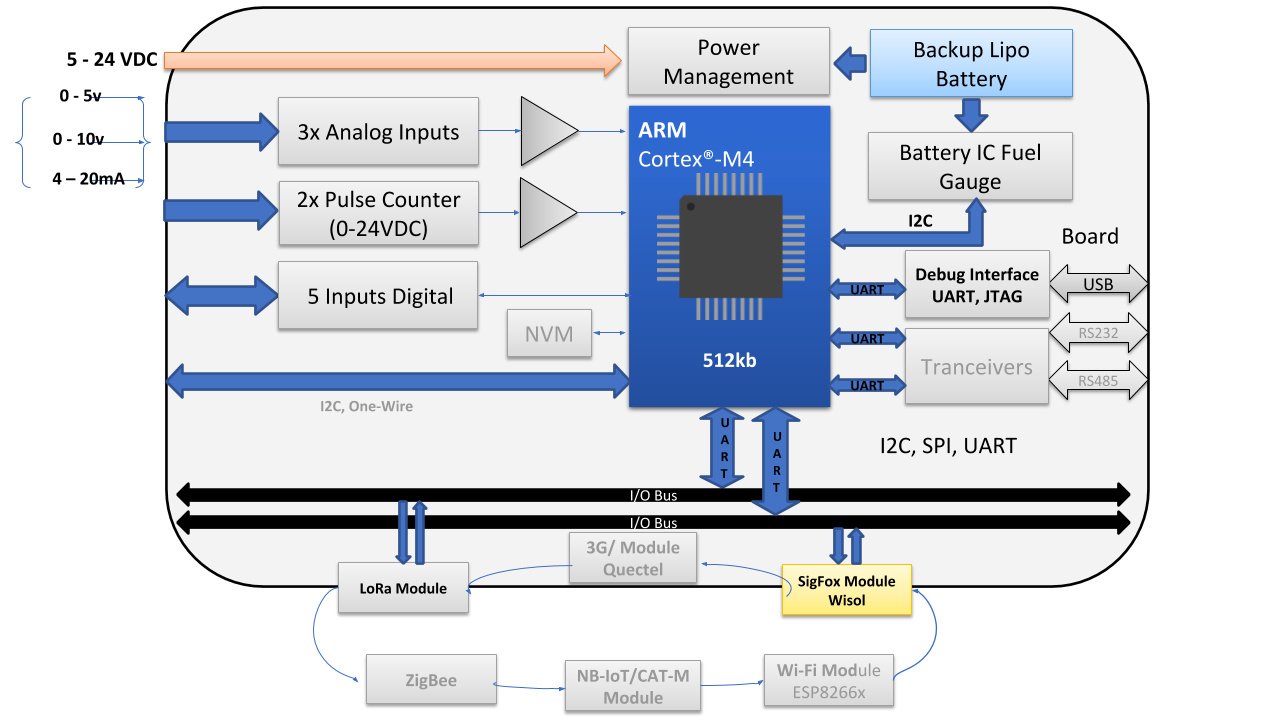
\includegraphics[scale=.35]{./Figures/esquemaGeneral.png}

	\caption{Diagrama general del sistema.}

	\label{fig:esquemaGeneral}

\end{figure}


El sistema consta de un medidor de voltaje para batería de LiPo, dos entradas analógicas de tensión, una de corriente y cinco entradas digitales con el fin de poder adquirir datos de diferentes variables en los procesos industriales. El dispositivo esta diseñado para tener diferentes funcionalidades sin embargo debido a la delimitación del alcance del trabajo no se implementaron los subsistemas que se observan en gris en la figura \ref{fig:esquemaGeneral}.


\section{Requerimientos}
Los siguientes son los requerimientos del presente trabajo:

\textbf{Grupo de requerimientos asociados al hardware:}
\begin{enumerate}

	\item Microcontrolador.

	\begin{itemize}

		\item Debe tener procesador ARM Cortex M0+ o M4.

		\item Debe tener 3 puertos UART.

		\item Debe tener comunicación I2C/SPI.

		\item Debe tener memoria flash mayor a 64 kb.

		\item Debe tener 3 entradas analógicas.

		\item Debe tener 5 entradas digitales.

	\end{itemize}

	%\item Nivel de protección debe ser IP65.

	\item Autonomía de la batería debe ser de 1 día.

	\item Módulo Sigfox.

		\begin{itemize}

			\item Debe tener un módulo \textit{Dual Zone} con comunicación por UART.

			\item Debe tener antena externa con centro de banda en 915 MHz.

		\end{itemize}

	\item Módulo Lora.

		\begin{itemize}

			\item Debe tener un módulo con comunicación por UART/I2C.

			\item Debe tener antena externa con centro de banda en 915 MHz.

		\end{itemize}

		\item El sistema debe tener una (1) entrada analógica de voltaje de 0-5 Vdc.
		
		\item El sistema debe tener una (1) entrada analógica de voltaje de 0-10 Vdc.

		\item El sistema debe tener una (1) entradas analógicas de corriente 4-20 mA.

		\item El sistema debe tener cinco (5) entradas digitales 3.3-24 Vdc.

\end{enumerate}



\textbf{Grupo de requerimientos asociados al módulo Sigfox:}

	\begin{enumerate}

		\item Debe colocarse en modo de bajo consumo mientras no esté en uso.

		\item Verificación de cada respuesta de comando AT enviado desde el MCU al módulo SIgFox.

	\end{enumerate}





\textbf{Grupo de requerimientos asociados al módulo Lora:}

	\begin{enumerate}

		\item Verificación de cada respuesta de los comandos enviados desde el MCU al módulo Lora.

		\item Debe colocarse en modo de bajo consumo mientras no esté en uso.

	\end{enumerate}



\textbf{Otros requerimientos:}

\begin{enumerate}

	\item En el sistema se podrán configurar umbrales máximos y mínimos de las lecturas analógicas.

	\item El sistema deberá verificar las entradas analógicas cada 1 minuto (parámetro configurable).

	\item El sistema saldrá del modo de bajo consumo cada vez que ocurra una interrupción por tiempo.

\end{enumerate}


%https://www.sigfox.com/en/sigfox-iot-radio-technology
\subsection{Sigfox}
Fundada en Francia en 2010 con el fin de construir una red global que se dedicara al Internet de las cosas y operara con un costo muy bajo y un consumo mínimo de energía. La tecnología Sigfox se basa en una comunicación por radio de largo alcance, dedicada por completo a hacer que cualquier objeto se comunique con muy bajo consumo de energía, extrayendo y transportando mensajes muy pequeños.

%https://build.sigfox.com/sigfox#coverage
El protocolo Sigfox se centra en: 
\begin{itemize}
    \item La autonomía: Consumo de energía extremadamente bajo, lo que permite años de duración de la batería.
    \item Simplicidad:  Sin configuración, solicitud de conexión o señalización. ¡El dispositivo está en funcionamiento en minutos!
    \item Eficiencia de precio: Desde el hardware utilizado en los dispositivos hasta la red, optimiza cada paso para que sea lo más rentable posible.
    \item Pequeños mensajes: No permiten activos o medios grandes en la red, solo notificaciones pequeñas: hasta 12 bytes ascendentes y 8 bytes descendentes.
    \item Complementariedad: Gracias al bajo costo y facilidad de configuración, también se puede usar Sigfox como una solución secundaria para cualquier otro tipo de red, como: WiFi, Bluetooth, GPRS, etc.
\end{itemize}

Como se puede observar en la figura \ref{fig:SigfoxOverview} El ciclo de vida de un mensaje de Sigfox es siguiente:
\begin{enumerate}
    \item Un dispositivo se despierta y emite un mensaje usando su antena de radio,
    \item Múltiples estaciones base de Sigfox en el área reciben el mensaje,
    \item Las estaciones base envían el mensaje a la nube de Sigfox,
    \item La nube de Sigfox envía el mensaje a la plataforma de el cliente.
\end{enumerate}

\begin{figure}[h]
	\centering
	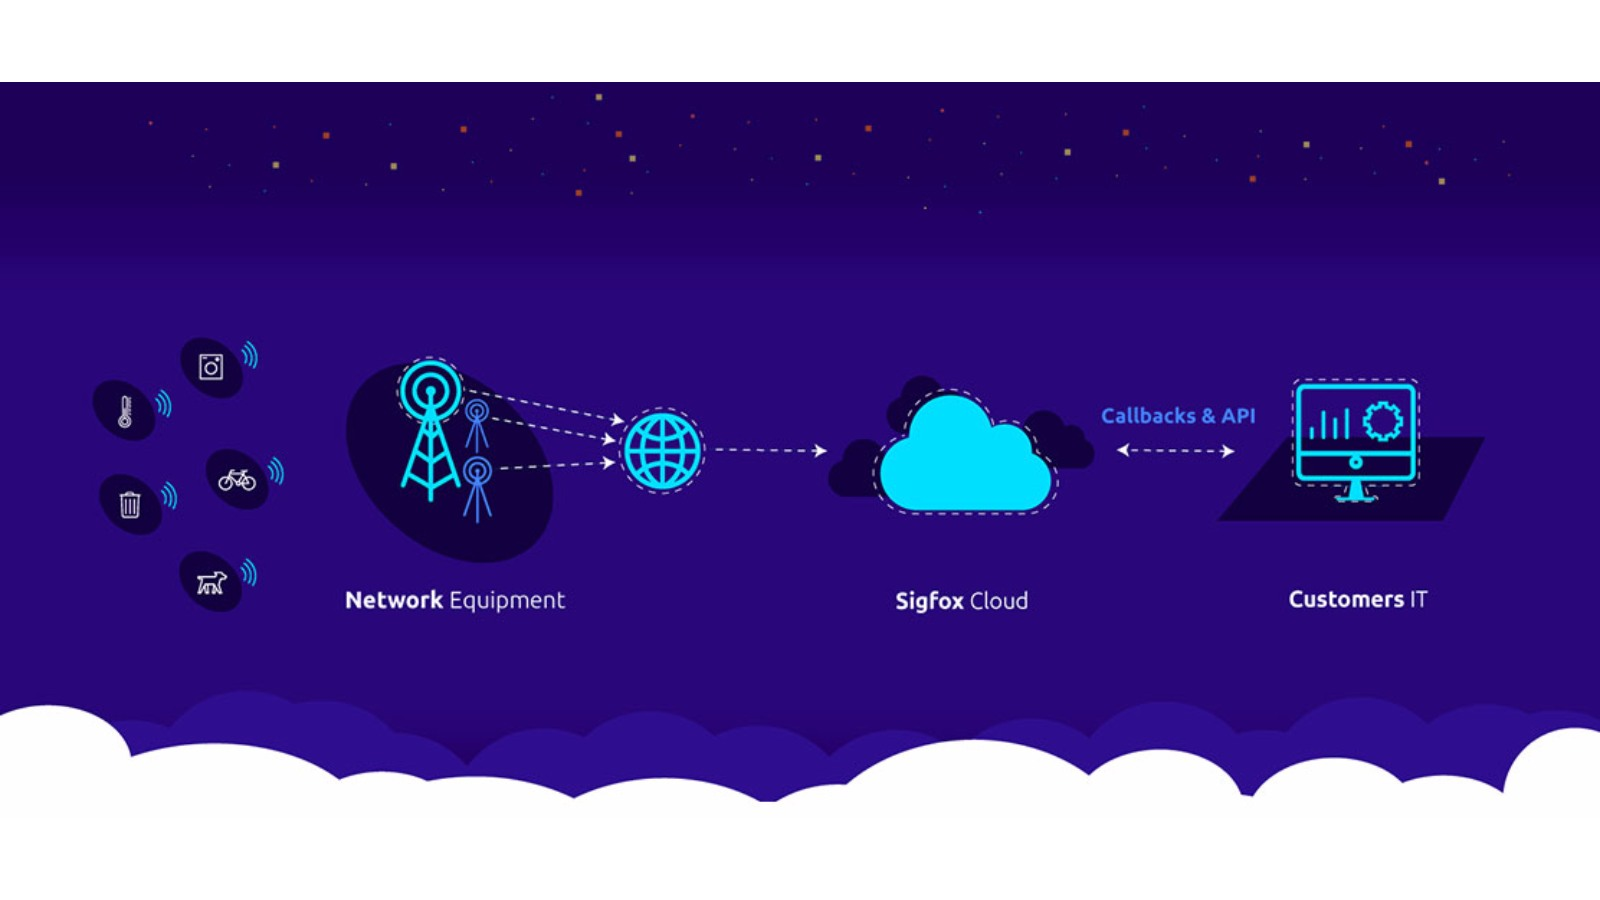
\includegraphics[scale=.25]{./Figures/SigfoxOverview.jpg}
	\caption{Ciclo de vida de un mensaje en Sigfox.}
	\label{fig:SigfoxOverview}
\end{figure}


Sigfox utiliza la tecnología de radio UNB y opera en las bandas sin licencia ISM (\textit{ industrial, scientific and medical}) para intercambiar mensajes de radio a través del aire en las frecuencias 868 MHz y 902-928 MHz. En cada pais, las  bandas ISM están bajo el control de las regulaciones locales, que definen restricciones técnicas para el uso del espectro, Sigfox tiene definidas configuraciones de radio que cumplan con las regulaciones locales.

%La modulación por desplazamiento de fase o PSK (Phase Shift Keying) es una forma de modulación angular que consiste en hacer variar la fase de la portadora entre un número determinado de valores discretos. La diferencia con la modulación de fase convencional (PM) es que mientras en ésta la variación de fase es continua, en función de la señal moduladora, en la PSK la señal moduladora es una señal digital y, por tanto, con un número de estados limitado.%

%https://www.link-labs.com/blog/sigfox-vs-lora
Sigfox combina UNB con modulación  DBPSK (\textit{differential binary phase shift keying}), este un método de transmisión de radio estándar que toma fragmentos de espectro muy estrechos y cambia la fase de la onda de radio portadora para codificar los datos. Esto permite que el receptor solo escuche en una pequeña porción de espectro, lo que mitiga el efecto del ruido. cada mensaje tiene un ancho de 100 Hz y se transfiere a una velocidad de 100 o 600 bits por segundos, dependiendo de la región \cite{RSpec}. %https://build.sigfox.com/sigfox-device-radio-specifications

Tiene una funcionalidad bidireccional, pero la capacidad para ir desde la estación base hasta el dispositivo final está restringida, y tendrá menos presupuesto de enlaces que hacia abajo. Esto se debe a que la sensibilidad del receptor en el dispositivo final no es tan buena como en la estación base.

%https://build.sigfox.com/sigfox-radio-configurations-rc
Sigfox tiene una red de cobertura global, que opera en la banda ISM en todo el mundo, las operaciones globales se dividen actualmente en seis  zonas geográficas, cada zona tiene un conjunto diferente de parámetros que acotan claramente la implementación del hardware del dispositivo, principalmente rango de frecuencia y potencia máxima irradiada. En la tabla \ref{tab:ZonasSigfox} se puede observar algunos de estos parámetros \cite{RConfg}.

\begin{table}[h]
	\centering
	\caption[Zonas de frecuencia]{Frecuencias según zonas}
	\begin{tabular}{l c c c c c c}    
		\toprule
		\textbf{ } 	   & \textbf{RC1} & \textbf{RC2} 	& \textbf{RC3}  & \textbf{RC4}   & \textbf{RC5}	& \textbf{RC6} \\
		\midrule
		Frecuencia central \textit{uplink} ( MHz)	    & 868.130 	& 902.200	&923.200  &920.800	&923.300 &865.200\\	
		Frecuencia central \textit{downlink} ( MHz) 	& 869.525	& 905.200   &922.200 &922.300	&922.300	&866.300\\
		Velocidad de datos \textit{uplink} ( bits/s)	& 100       &600        &100     &600       &100        &100\\	
		Velocidad de datos \textit{downlink} ( bits/s)	& 600       & 600    	&600     & 600       & 600    	&600\\
		EIRP (dBm)		                             	 & 16       & 24		&16     &24	        &14         &16\\
		\bottomrule
		\hline
	\end{tabular}
	\label{tab:ZonasSigfox}
\end{table}

Las 6 zonas  actuales con la configuración de radio de Sigfox son:
\begin{itemize}
    \item RC1:
        \begin{itemize}
            \item Europa: Bélgica, Croacia, República Checa, Dinamarca, Estonia, Finlandia, Francia, Alemania, Hungría, Irlanda, Italia, Luxemburgo, Malta, Países Bajos, Noruega, Polonia, Portugal, Eslovaquia, España, Suecia, Suiza, Reino Unido.
            \item Francia de ultramar: Guayana Francesa, Polinesia Francesa, Guadalupe, Martinica, Mauricio, Mayotte, Nueva Caledonia, Reunión.
            \item Oriente Medio y África: Irán, Kenia, Omán, Sudáfrica, Túnez, Emiratos Árabes Unidos.
        \end{itemize}
    \item RC2:
        \begin{itemize}
            \item Brasil, Canadá, México, Puerto Rico, Estados Unidos.
        \end{itemize}
    \item RC3:
        \begin{itemize}
            \item Japón
        \end{itemize}
    \item RC4:
        \begin{itemize}
            \item América Latina: Argentina, Chile, Colombia, Costa Rica, Ecuador, El Salvador, Guatemala, Honduras, Panamá, Perú, Uruguay.
            \item Asia Pacífico: Australia, Hong Kong, Malasia, Nueva Zelanda, Singapur, Taiwán, Tailandia.
        \end{itemize}
    \item RC5:
        \begin{itemize}
            \item Corea del Sur
        \end{itemize}
    \item RC6:
        \begin{itemize}
            \item India
        \end{itemize}
\end{itemize}

En la figura \ref{fig:coverageSigfox} se puede observar el mapa de cobertura de Sigfox.

\begin{figure}[h]
	\centering
	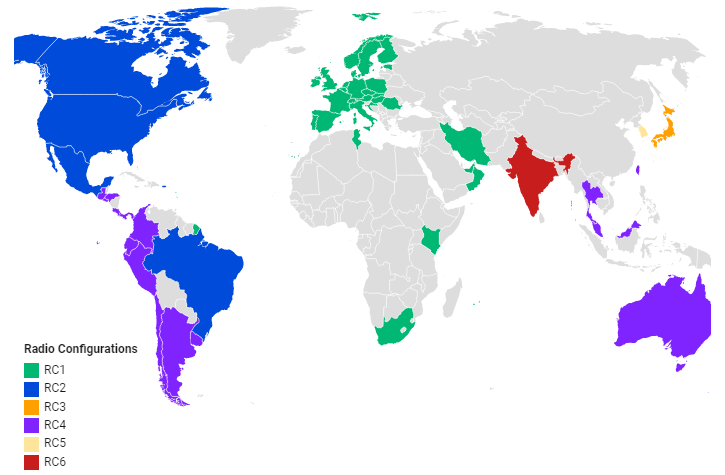
\includegraphics[scale=.65]{./Figures/coverageSigfox.PNG}
	\caption{Disponibilidad geográfica de Sigfox\protect\footnotemark.}
	\label{fig:coverageSigfox}
\end{figure}
\footnotetext{\url{https://build.sigfox.com/sigfox-radio-configurations-rc}}
%https://build.sigfox.com/certification
La Certificación Sigfox es el reconocimiento de la conformidad de un dispositivo con las especificaciones de certificación Sigfox para garantizar la compatibilidad con los servicios Sigfox y el rendimiento nominal en la red. La certificación Sigfox \textit{Ready} es obligatoria para que cualquier dispositivo esté conectado a la red Sigfox, con la excepción de las soluciones de desarrollo ( prototipos).

Sigfox requiere la certificación para los dispositivos que desean comunicarse en la red Sigfox. Esto es para garantizar la interoperabilidad y la prestación de servicios a un nivel de rendimiento nominal. Al finalizar el proceso de certificación, Sigfox otorga un certificado al cliente. Este certificado es necesario para registrar cualquier dispositivo del mismo modelo en la red Sigfox.

La certificación Sigfox \textit{Ready} se clasifica en clases, en la  siguiente tabla \ref{tab:Tecno} se observan las características\cite{CertificationSigfox}.
%https://storage.sbg1.cloud.ovh.net/v1/AUTH_669d7dfced0b44518cb186841d7cbd75/dev_medias/build/40599x1josfx0hz/Sigfox%20device%20cookbook%20-%20communication%20configuration%20Nov%202018.pdf
\begin{table}[h]
	\centering
	\caption[Sigfox \textit{Ready}]{Caracteristicas de certificación (\textit{Sigfox Device Class}) }
	\begin{tabular}{l c c c}    
		\toprule
		\textbf{  } & \multicolumn{3}{c}{\textit{Device EIRP}} \\ \cline{2-4} 
		\textbf{ \textit{Device Class} } & \textbf{RC1, RC3} & \textbf{RC2,RC4} 	& \textbf{RC5} \\
		\midrule
		0u	    &$\ge12$ dBm 	&$\ge20$ dBm & $\ge10$ dBm \\	
		1u	&$\ge7$ and <12 dBm &$\ge15$ and <20 dBm & $\ge5$ and <10 dBm\\
		2u	&$\ge2$ and <7 dBm & $\ge10$ and <15 dBm & $\ge0$ and <5 dBm \\	
		3u	&< 2 dBm &< 10 dBm &< 0 dBm   \\
		\bottomrule
		\hline
	\end{tabular}
	\label{tab:ZonasSigfox}
\end{table}
%https://storage.sbg1.cloud.ovh.net/v1/AUTH_669d7dfced0b44518cb186841d7cbd75/dev_medias/build/40599x1josfx0hz/Sigfox%20device%20cookbook%20-%20communication%20configuration%20Nov%202018.pdf

La figura \ref{fig:certificacion} muestra la prioridad de las clases, siendo clase 0u la de mayor potencia de transmisión\cite{CertificationSigfox}.
\begin{figure}[h]
	\centering
	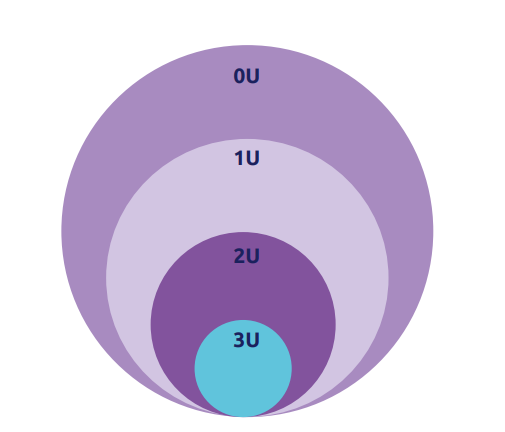
\includegraphics[scale=.65]{./Figures/certificacion.PNG}
	\caption{Potencia según clases.}
	\label{fig:certificacion}
\end{figure}

%https://www.sigfox.com/en/coverage 
Sigfox se basa en una infraestructura privada de antenas y servidores, la red es desplegada por un operador local, En América es la empresa WND \textit{group } (\textit{Wireless Network Development}) , la cual se encuentra en Colombia, Argentina, Brasil, Chile, Costa Rica, Ecuador, El Salvador, Mexico, Panamá y United Kingdom.Tambien existen los canales que son los encargados de consumir y ofrecer el servicio que brinda WND \cite{SigfoxCoverage}. 
%https://build.sigfox.com/backend-callbacks-and-api

La información se maneja en un servidor Sigfox  \textit{back-end} donde el usuario tiene la posibilidad darle un tratamiento a la información a través de una interfaz API (\textit{Application Programming Interface}). En la plataforma de Sigfox, una empresa suele estar representada por un "Grupo", que contiene "Tipo de dispositivo". Cada tipo de dispositivo puede atribuirse a una "familia" de dispositivos como se observa en la figura \ref{fig:backendSigfox}. Todas las unidades del mismo producto se agruparán como un tipo de dispositivo para permitir que todas se comporten exactamente de la misma manera cuando la red Sigfox recibe un mensaje. 
%https://build.sigfox.com/backend-callbacks-and-api
\begin{figure}[h]
	\centering
	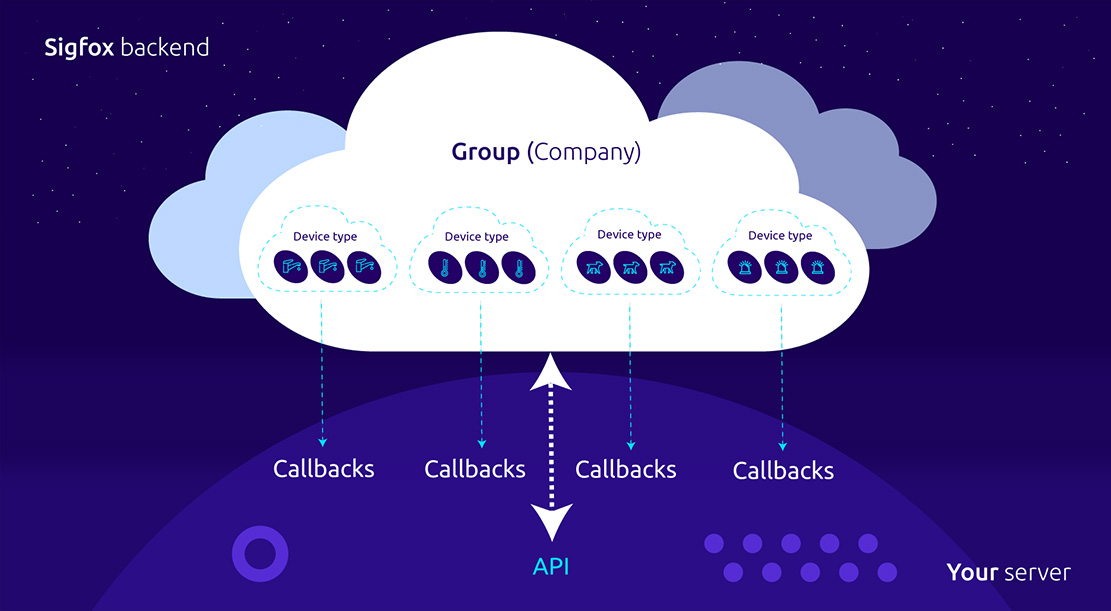
\includegraphics[scale=.35]{./Figures/backendSigfox.jpg}
	\caption{Diagrama Sigfox \textit{back-end} \protect\footnotemark}
	\label{fig:backendSigfox}
\end{figure}
\footnotetext{\url{https://build.sigfox.com/backend-callbacks-and-api}}

Sigfox basa su modelo de negocio en conectividad, ofrece servicios de comunicación seguros, bidireccionales y listos para usar, para conectar los dispositivos a la nube. Existen planes de conectividad anuales que difieren en la cantidad de mensajes que pueden transmitir al día, máximo 140 mensajes \textit{uplink} y 4 mensajes \textit{downlink}.Los mensajes de bajada (\textit{downlink}) siempre están precedidos por un mensaje ascendente, en cualquier otro momento que el servidor quiera enviar un mensaje descendente debe esperar hasta la siguiente transmisión de un mensaje ascendente (\textit{uplink}).

%LoRa Alliance. White Paper: A Technical Overview of Lora and Lorawan; The LoRa Alliance: San Ramon, CA,USA, 2015.
\subsection{LoRa}
LoRa, el cual es el acrónimo de \textit{"Long Range"}, es un sistema de comunicaciones inalámbricas de largo alcance, originalmente fue desarrollada por Semtech y actualmente es promovida por LoRa \textit{Alliance}.

LoRa esta basada en dos capas distintas, como se puede observar en la figura \ref{fig:LoraStack}: 
\begin{enumerate}
    \item Capa física que utiliza la técnica de modulación  de radio CSS (\textit{Chirp Spread Spectrum})\cite{CSS}.
    \item LoRaWAN un protocolo de capa MAC (\textit{Medium Acces Control}).
\end{enumerate}

\begin{figure}[h]
	\centering
	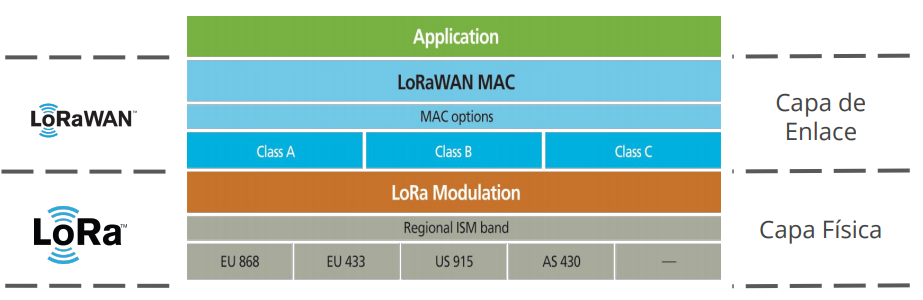
\includegraphics[scale=.55]{./Figures/LoraWanClasses.PNG}
	\caption{LoraWan Stack\protect\footnotemark.}
	\label{fig:LoraStack}
\end{figure}
\footnotetext{\url{https://www.tuv.com/media/corporate/products_1/electronic_components_and_lasers/TUeV_Rheinland_Overview_LoRa_and_LoRaWANtmp.pdf}}
%En las comunicaciones digitales, el espectro de propagación de chirrido ( CSS ) es una técnica de espectro ensanchado que utiliza pulsos de chirrido modulados en %frecuencia de banda ancha para codificar información. [1] Un chirrido es una señal sinusoidal de aumento o disminución de la frecuencia con el tiempo (a menudo con %una expresión polinomial para la relación entre el tiempo y la frecuencia). En la imagen se muestra un ejemplo de un cambio de tendencia en el que la frecuencia %aumenta linealmente con el tiempo. A veces, la frecuencia de los upchirps aumenta exponencialmente con el tiempo.
%Al igual que con otros métodos de espectro ensanchado, el espectro de chirrido utiliza todo su ancho de banda asignado para transmitir una señal, lo que lo hace %robusto al ruido del canal. Además, debido a que los chirridos utilizan una amplia banda del espectro, el espectro extendido de los chirridos también es resistente %al desvanecimiento de múltiples vías, incluso cuando se opera a una potencia muy baja. Sin embargo, es diferente del espectro extendido de secuencia directa (DSSS) %o del espectro expandido de salto de frecuencia (FHSS), ya que no agrega ningún elemento pseudoaleatorio a la señal para ayudar a distinguirlo del ruido en el %canal, sino que se basa en el Naturaleza lineal del pulso chirrido. Además, el espectro del chirrido es resistente al efecto Doppler., lo que es típico en %aplicaciones de radio móvil. [2]

La capa física LoRa, permite aplicaciones de largo alcance, baja potencia y comunicaciones de bajo rendimiento. Opera en las bandas ISM de 433 MHz, 868 MHz o 915 MHz, esto depende de la región en la que se despliegue la red. La carga útil de cada transmisión puede oscilar entre 2 y 255 octetos, la velocidad de datos puede alcanzar hasta 50 Kbps cuando se emplea la adición de canales. Esta técnica de modulación es una tecnología patentada por Semtech\cite{FEHRI20181096}.

%https://lora-alliance.org/sites/default/files/2018-05/2015_-_lorawan_specification_1r0_611_1.pdf
%LoraWanClasses.PNG

%LoRa Alliance. White Paper: A Technical Overview of Lora and Lorawan; The LoRa Alliance: San Ramon, CA,USA, 2015.
%https://www.tuv.com/media/corporate/products_1/electronic_components_and_lasers/TUeV_Rheinland_Overview_LoRa_and_LoRaWANtmp.pdf
LoRaWAN define el protocolo de comunicación y la arquitectura del sistema para la red mientras que la capa física LoRa permite el enlace de comunicación de largo alcance.
El protocolo y la arquitectura de red tienen la mayor influencia para determinar la duración de la batería de un nodo, la capacidad de la red, la calidad del servicio, la seguridad, y la variedad de aplicaciones servidas por la red. 

La arquitectura red es una topología estrella de largo alcance (\textit{star-of-stars}) en la que las puertas de enlace (\textit{gateways}) retransmiten los mensajes de los dispositivos finales. Es decir los nodos no están asociados con una puerta de enlace específica. En lugar, los datos transmitidos por un nodo normalmente son recibidos por múltiples puertas de enlace. Cada puerta de enlace reenviará el paquete recibido desde el nodo final al servidor de red a través de una interfaz de red de retorno (\textit{backhaul}) (ya sea 3G, Ethernet, satélite o WiFi). Ver figura \ref{fig:Loraarquitecturenetwork}.

\begin{figure}[h]
	\centering
	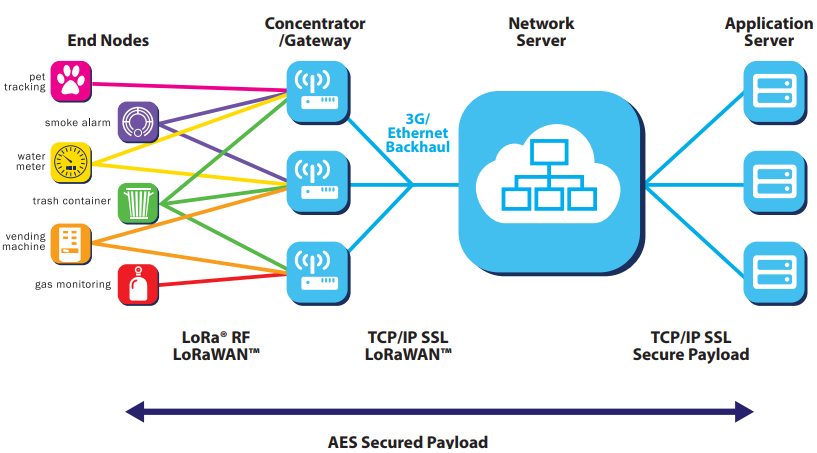
\includegraphics[scale=.70]{./Figures/Loraarquitecturenetwork.PNG}
	\caption{LoRa arquitectura de red\protect\footnotemark.}
	\label{fig:Loraarquitecturenetwork}
\end{figure}
\footnotetext{\url{https://www.tuv.com/media/corporate/products_1/electronic_components_and_lasers/TUeV_Rheinland_Overview_LoRa_and_LoRaWANtmp.pdf}}

La comunicación entre los nodos generalmente es bidireccional, la puerta de enlace se distrbuye en diferentes frecuencias, canales y tarifas de datos. Las tasas de datos de LoRa varían de 0.3 Kbps a 50Kbps, Para  maximizar la duración de batería de los dispositivos finales como la capacidad general de la red, la red LoRa gestiona la velocidad de datos y la salida de RF para cada dispositivo final individualmente\protect\footnotemark.
\footnotetext{\url{https://lora-alliance.org/sites/default/files/2018-05/2015_-_lorawan_specification_1r0_611_1.pdf}}


Los dispositivos finales pueden transmitir en cualquier canal disponible en cualquier momento, siempre y cuando se respeten las siguientes reglas:
\begin{itemize}
    \item El dispositivo final cambia el canal de forma pseudoaleatoria para cada  transmisión. La diversidad de frecuencia resultante hace que el sistema sea más robusto para interferencias.
    \item El dispositivo final respeta el ciclo de trabajo de transmisión máximo en relación con los reglamentos de la sub-banda usados y locales.
    \item El dispositivo final respeta la duración máxima de transmisión (o tiempo de permanencia) en relación con la sub-banda utilizada y las normativas locales.
\end{itemize}

%FALATA HABLAR DE TEOREMA SHANON HARTLEY, ANCHO DE BANDA Y EL RUUIDO, SALTO DE FRECUENCIA Y DSSS EXPECTRO EXPANDIDO-SECUENCIA DIRECTA


loRAWAN Clases :

La red  LoRa distingue entre  tres clases bidireccionales: clase A, clase B, clase C. estas tres clases se usan para diferentes aplicaciones y tienen una variedad de requisitos para optimizar una variedad de aplicaciones finales. Las clases intercambian la latencia de comunicación del enlace descendente frente a la duración de la batería. ver figura \ref{fig:Loracomparacionclases}.

\begin{figure}[h]
	\centering
	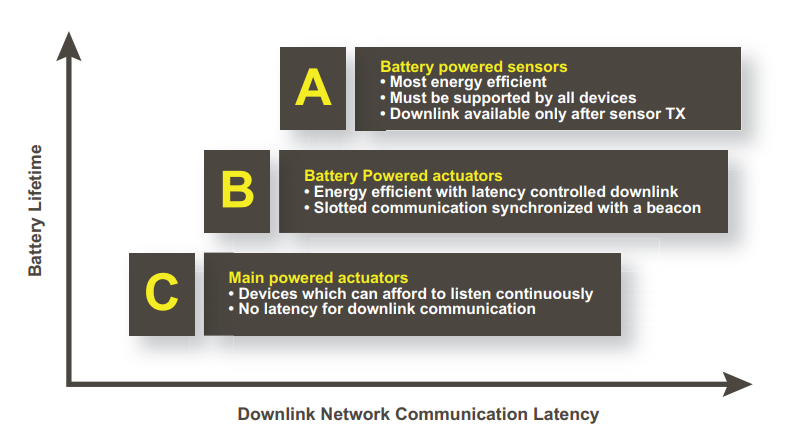
\includegraphics[scale=.65]{./Figures/Loracomparacionclases.PNG}
	\caption{LoraWan clases\protect\footnotemark.}
	\label{fig:Loracomparacionclases}
\end{figure}
\footnotetext{\url{https://www.tuv.com/media/corporate/products_1/electronic_components_and_lasers/TUeV_Rheinland_Overview_LoRa_and_LoRaWANtmp.pdf}}


\begin{itemize}
    \item Clase A, bidireccional: los dispositivos finales de Clase A pueden programar una transmisión de enlace ascendente en función de las necesidades propias con una pequeña variación basada en una base de tiempo aleatorio (ALOHA -type of protocol)., esta clase de dispositivos permite comunicaciones bidireccionales, por lo que a cada transmisión de enlace ascendente le siguen dos ventanas cortas de recepción. La transmisión del enlace descendente desde el servidor en cualquier otro momento tiene que esperar hasta que ocurra la siguiente transmisión de enlace ascendente. Los dispositivos de clase A tienen el menor consumo de energía, pero también ofrecen menos flexibilidad en las transmisiones de enlace descendente. Ver figura \ref{fig:LoraclassA}.

    \item Clase B, bidireccional con ranuras de recepción programadas: Los dispositivos finales de Clase B  tienen ventanas extras de recepción  abiertos a unas horas programadas. Por lo tanto, se requiere una baliza sincronizada desde el servidor, de modo que
    El servidor pueda saber cuándo está escuchando el dispositivo final. Ver figura \ref{fig:LoraClaseB}.
    
    \item Clase C, bidireccional con ranuras de recepción máximas: los dispositivos finales de Clase C tienen casi todo el tiempo ventanas de recepción continuas, de esta forma tienen el máximo consumo de energía. Ver figura \ref{fig:LoraClaseC}.
\end{itemize}


\begin{figure}[h]
	\centering
	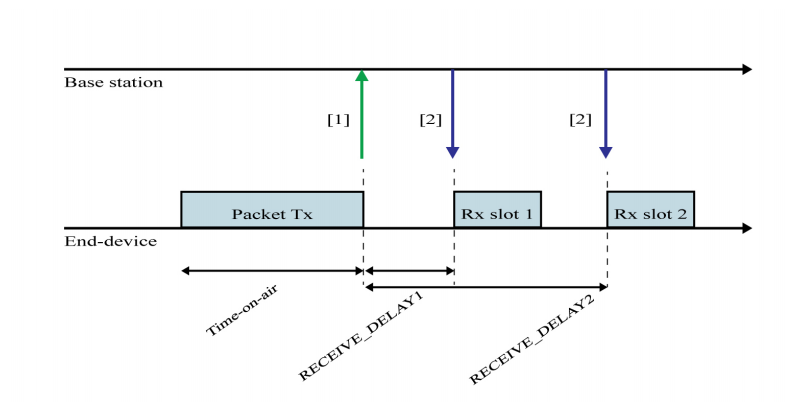
\includegraphics[scale=.65]{./Figures/LoraclassA.PNG}
	\caption{Clase A \protect\footnotemark.}
	\label{fig:LoraclassA}
\end{figure}
\footnotetext{\url{https://upcommons.upc.edu/handle/2117/98853}}

\begin{figure}[h]
	\centering
	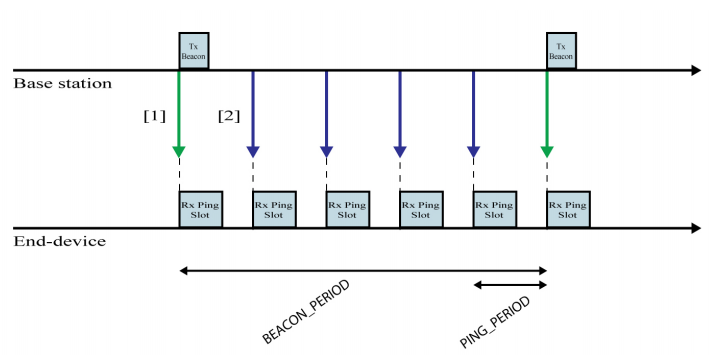
\includegraphics[scale=.65]{./Figures/LoraClaseB.PNG}
	\caption{Clase B \protect\footnotemark.}
	\label{fig:LoraClaseB}
\end{figure}
\footnotetext{\url{https://upcommons.upc.edu/handle/2117/98853}}

\begin{figure}[h]
	\centering
	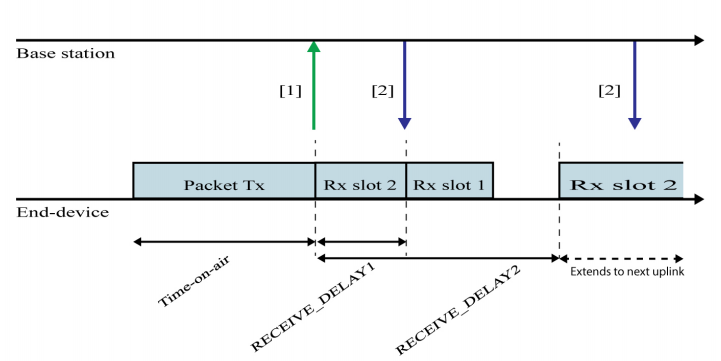
\includegraphics[scale=.65]{./Figures/LoraClaseC.PNG}
	\caption{Clase C \protect\footnotemark.}
	\label{fig:LoraClaseC}
\end{figure}
\footnotetext{\url{https://upcommons.upc.edu/handle/2117/98853}}


%-----------------------------

% \subsection{Ecuaciones}
% \label{sec:Ecuaciones}

% Al insertar ecuaciones en la memoria estas se deben numerar de la siguiente forma:

% \begin{equation}
% 	\label{eq:metric}
% 	ds^2 = c^2 dt^2 \left( \frac{d\sigma^2}{1-k\sigma^2} + \sigma^2\left[ d\theta^2 + \sin^2\theta d\phi^2 \right] \right)
% \end{equation}
                                                        
% Es importante tener presente que en el caso de las ecuaciones estas pueden ser referidas por su número, como por ejemplo ``tal como describe la ecuación \ref{eq:metric}'', pero también es correcto utilizar los dos puntos, como por ejemplo ``la expresión matemática que describe este comportamiento es la siguiente:''

% \begin{equation}
% 	\label{eq:schrodinger}
% 	\frac{\hbar^2}{2m}\nabla^2\Psi + V(\mathbf{r})\Psi = -i\hbar \frac{\partial\Psi}{\partial t} \geq
% \end{equation}

% Para las ecuaciones se debe utilizar un tamaño de letra equivalente al utilizado para el texto del trabajo, en tipografía cursiva y preferentemente del tipo Times New Roman o similar. El espaciado antes y después de cada ecuación es de aproximadamente el doble que entre párrafos consecutivos del cuerpo principal del texto. Por suerte la plantilla se encarga de esto por nosotros.

% Para generar la ecuación \ref{eq:metric} se utilizó el siguiente código:

% \begin{verbatim}
% \begin{equation}
% 	\label{eq:metric}
% 	ds^2 = c^2 dt^2 \left( \frac{d\sigma^2}{1-k\sigma^2} + 
% 	\sigma^2\left[ d\theta^2 + 
% 	\sin^2\theta d\phi^2 \right] \right)
% \end{equation}
% \end{verbatim}

% Y para la ecuación \ref{eq:schrodinger}:

% \begin{verbatim}
% \begin{equation}
% 	\label{eq:schrodinger}
% 	\frac{\hbar^2}{2m}\nabla^2\Psi + V(\mathbf{r})\Psi =
% 	-i\hbar \frac{\partial\Psi}{\partial t}
% \end{equation}

% \end{verbatim}